\documentclass[final]{article}

\PassOptionsToPackage{numbers, compress}{natbib} % numbered citations for IEEE style
\usepackage{aps360}
\makeatletter\renewcommand{\@noticestring}{}\makeatother % remove NeurIPS footer from course style
\usepackage[utf8]{inputenc}
\usepackage[T1]{fontenc}
\usepackage{hyperref}
\usepackage{url}
\usepackage{booktabs}
\usepackage{amsmath}
\usepackage{amsfonts}
\usepackage{nicefrac}
\usepackage{microtype}
\usepackage{xcolor}
\usepackage{graphicx}
\graphicspath{{figures/}{./}}
\usepackage{tikz}
\usetikzlibrary{positioning,arrows.meta,fit,backgrounds,calc}

\setlength{\textfloatsep}{8pt plus 2pt minus 2pt}
\setlength{\intextsep}{6pt plus 2pt minus 2pt}
\setlength{\abovecaptionskip}{3pt}
\setlength{\belowcaptionskip}{0pt}

\title{Connected Markets: Predicting Stock Returns\\with Graph Neural Networks\\[2pt]{\large Project Progress Report}}

\author{%
  Kabir Jain \\
  Student Number: 1010339242\\
  Email: \href{mailto:kabir.jain@mail.utoronto.ca}{kabir.jain@mail.utoronto.ca}\\
  \href{https://colab.research.google.com/drive/1BibeXLFHFts0R9ro75Up_cdv6xue14fy}{Google Colab notebook}\\
  \href{https://github.com/Kabirjain01/Connected-Markets}{GitHub repository}\\
}

\begin{document}

\maketitle

\vspace{-0.45in}

\section*{Brief Project Description}
Companies are linked: when a large customer has a bad quarter, its suppliers often fall days later, and prices absorb such news only gradually \cite{cohen2008economic}. My project tests whether knowing how companies are connected improves next-week stock return predictions. Its input is the last 20 trading days of returns and volume changes for 100 large U.S.\ stocks, plus a graph linking stocks that share a sector or moved together over the past year. Its output is a score ranking every stock against the other 99 for the coming week. Deep learning suits this because it combines sequences, which an LSTM reads day by day, with an irregular network of companies, which a graph neural network (GNN) is designed for \cite{feng2019temporal, kim2019hats, xu2021hist}.

\begin{figure}[!ht]
  \centering
  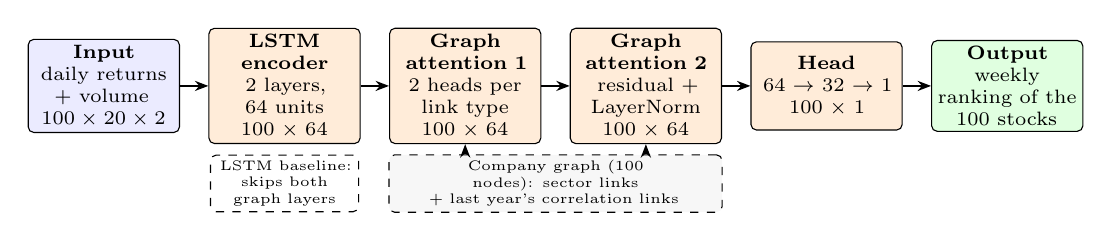
\begin{tikzpicture}[
      font=\scriptsize,
      b/.style={draw, rounded corners=2pt, align=center, text width=1.78cm, minimum height=1.12cm, inner sep=2pt, execute at begin node={\hyphenpenalty10000\relax}},
      arr/.style={-{Stealth[length=1.7mm]}, thick}
    ]
    \node[b, fill=blue!8] (x) {\textbf{Input}\\daily returns + volume\\$100 \times 20 \times 2$};
    \node[b, fill=orange!15, right=0.36cm of x] (l) {\textbf{LSTM encoder}\\2 layers, 64 units\\$100 \times 64$};
    \node[b, fill=orange!15, right=0.36cm of l] (g1) {\textbf{Graph attention 1}\\2 heads per link type\\$100 \times 64$};
    \node[b, fill=orange!15, right=0.36cm of g1] (g2) {\textbf{Graph attention 2}\\residual + LayerNorm\\$100 \times 64$};
    \node[b, fill=orange!15, right=0.36cm of g2] (h) {\textbf{Head}\\$64 \rightarrow 32 \rightarrow 1$\\$100 \times 1$};
    \node[b, fill=green!12, right=0.36cm of h] (o) {\textbf{Output}\\weekly ranking of the 100 stocks};
    \draw[arr] (x) -- (l); \draw[arr] (l) -- (g1); \draw[arr] (g1) -- (g2); \draw[arr] (g2) -- (h); \draw[arr] (h) -- (o);
    \path let \p1 = (g1.west), \p2 = (g2.east) in
      node[draw, dashed, rounded corners=2pt, fill=gray!6, align=center, inner sep=2pt, font=\tiny,
           minimum width=\x2-\x1, text width=\x2-\x1-4pt] (adj) at ($(g1.south)!0.5!(g2.south) + (0,-0.5)$)
      {Company graph (100 nodes): sector links\\+ last year's correlation links};
    \draw[arr] (adj.north -| g1.south) -- (g1.south);
    \draw[arr] (adj.north -| g2.south) -- (g2.south);
    \node[draw, dashed, rounded corners=2pt, align=center, inner sep=2pt, font=\tiny, text width=1.74cm] (base) at ($(l.south) + (0,-0.5)$) {LSTM baseline: skips both graph layers};
  \end{tikzpicture}
  \caption{Implemented model with tensor shapes for one week (\textbf{78{,}273 parameters}). The LSTM baseline (52{,}801 parameters) skips the graph layers, isolating what the graph adds.}
  \label{fig:model}
\end{figure}

\section*{Notable Contribution}
\subsection*{Data Processing}
All code runs end to end in the linked Colab notebook in about 4 minutes on a GPU:
\begin{enumerate}
  \setlength{\itemsep}{1pt}\setlength{\parskip}{0pt}
  \item \textbf{Sources:} the current S\&P~500 table on Wikipedia gives 503 tickers with GICS sectors and SEC CIK numbers (500 after removing duplicate share classes such as GOOG). Daily split- and dividend-adjusted closes and volume from 2009-01-02 to 2026-11-20 come from \texttt{yfinance} (0 failed downloads).
  \item \textbf{Cleaning:} days when fewer than half the stocks traded are dropped (4{,}500 trading days remain). Non-positive prices become missing (no gaps needed filling), and stocks without a full history from January 2009 are dropped (88), leaving 412.
  \item \textbf{Universe:} the 100 stocks with the highest average daily dollar volume (price times shares traded) in 2009, which measures size using only information available at the start.
  \item \textbf{Samples:} every 5 trading days, each stock's input is its last 20 daily log returns and changes in log volume. Both are standardized with training-period statistics only (means 0.0004 and -0.0002, standard deviations 0.0167 and 0.365). The target is the next 5-day log return, ranked among the 100 stocks that week (-0.5 to +0.5), and labelled ``outperform'' if above that week's median.
  \item \textbf{Graph:} sector links join stocks in the same GICS sector (602 links). Correlation links join each stock to the 5 stocks most correlated with it over the previous 252 trading days, rebuilt every January from past data only (375 to 432 links per year).
  \item \textbf{Splits and checks:} train 2010 to 2019, validation 2020 to 2021, test 2022 onward, dropping weeks whose target crosses a boundary. The notebook checks that all inputs are finite and each week has 50 stocks per class.
\end{enumerate}

This gives \textbf{503 training weeks} (50{,}300 stock-weeks, 25{,}150 per class), \textbf{100 validation weeks} (10{,}000 stock-weeks) and 244 sealed test weeks. Half the correlation links cross sectors (Figure~\ref{fig:data}c).

\begin{figure}[!ht]
  \centering
  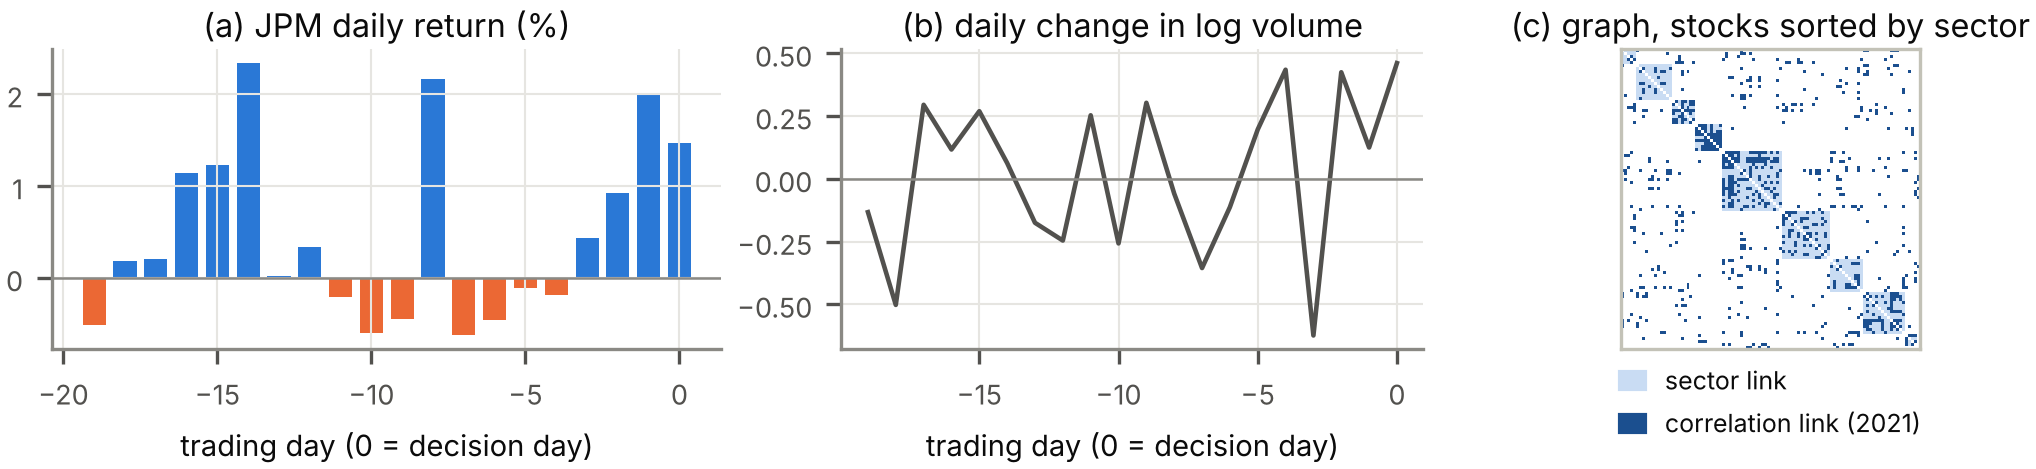
\includegraphics[width=\textwidth]{fig_data.png}
  \caption{(a, b) A cleaned training sample: 20 input days for JPM before 2017-06-29 (target: next-week return +3.47\%, ``outperform''). (c) The graph, stocks sorted by sector: light squares are sector links, dark squares correlation links.}
  \label{fig:data}
\end{figure}

\textbf{Testing on never-before-seen data:} the test years (2022 to 2026) stay sealed until the final report, and after freezing the model I will also test on new prices from December 2026 onward.

\textbf{Challenges:} Yahoo Finance limits download speed, so downloads are batched, retried and cached. Today's S\&P~500 list leaves out later-delisted companies (survivorship bias), which choosing stocks by 2009 activity reduces but does not remove.

\textbf{Supply-chain links (proposal feedback):} 10-K filings must name any customer above 10\% of revenue, but as the feedback noted, these mostly link small suppliers to large customers, so few may fall inside my universe. I have written and tested an EDGAR extraction that finds these sentences in each stock's 10-K for 2011, 2015, 2019 and 2023 and matches the customer to the universe. I will report verified edges per year, and if few fall inside the universe, allow one endpoint outside it.

\subsection*{Baseline Model}
Two baselines are hand-coded rules: momentum (20-day winners keep rising) and short-term reversal (5-day winners fall back). The main machine learning baseline is a ridge regression predicting the weekly rank from the 20 standardized daily returns, with only its regularization strength ($\alpha = 1000$) tuned on validation. Following the proposal feedback, I also trained it on the same 40 inputs as the LSTM (returns and volume changes) for a like-for-like comparison. The neural baseline is the LSTM without graph layers (Figure~\ref{fig:model}). All models are scored on validation by the information coefficient, $\text{IC} = \frac{1}{T}\sum_{t} \operatorname{SpearmanCorr}(\hat{s}_t, r_t)$, the average weekly rank correlation between the 100 predicted scores $\hat{s}_t$ and realized returns $r_t$ (0 means no skill), and by accuracy at picking outperformers (50\% is guessing). I also report the yearly return and Sharpe ratio of the 10 top-ranked stocks above the 100-stock average, before and after 0.10\% costs per trade.

\begin{table}[!ht]
  \centering
  \caption{Validation results (2020 to 2021). Seed s.d.: spread of IC across 3 seeds. Portfolio columns: top-10 stocks versus the 100-stock average, per year, with net Sharpe after costs.}
  \label{tab:results}
  \footnotesize
  \setlength{\tabcolsep}{2.9pt}
  \begin{tabular}{lrrrrrrrr}
\toprule
 & \multicolumn{4}{c}{Information coefficient (IC)} & & \multicolumn{3}{c}{Top-10 portfolio} \\
\cmidrule(lr){2-5}\cmidrule(lr){7-9}
Model & Train & Val & Seed s.d. & $t$-stat & Accuracy & Excess/yr & Sharpe & Net Sharpe \\
\midrule
Momentum (20-day rule) & -0.006 & +0.016 & n/a & +0.6 & 50.3\% & +4.4\% & +0.21 & -0.01 \\
Reversal (5-day rule) & +0.011 & -0.001 & n/a & 0.0 & 50.4\% & -3.4\% & -0.13 & -0.48 \\
Ridge, returns only & +0.028 & -0.038 & n/a & -1.7 & 48.8\% & -16.0\% & -0.82 & -1.31 \\
Ridge, returns + volume & +0.043 & -0.039 & n/a & -1.9 & 48.6\% & -6.9\% & -0.38 & -0.91 \\
\midrule
LSTM, no graph & +0.011 & +0.006 & 0.0042 & +0.2 & 50.5\% & +6.3\% & +0.33 & -0.14 \\
GNN, sector + correlation & +0.011 & +0.012 & 0.0100 & +0.6 & 50.9\% & -0.3\% & -0.02 & -0.50 \\
\midrule
GNN, sector links only & +0.014 & +0.011 & 0.0003 & +0.6 & 50.5\% & +15.9\% & +0.99 & +0.48 \\
GNN, correlation links only & +0.013 & \textbf{+0.020} & 0.0036 & +1.0 & 50.9\% & +12.9\% & +0.70 & +0.23 \\
\bottomrule
\end{tabular}
\end{table}

Ridge regression fits the training years (IC +0.0279) but fails on validation (\textbf{IC -0.0379}), and its top-10 portfolio finished 31\% behind the average over two years. Adding volume does not help (validation IC -0.039), so the inputs are not why it fails. The two rules stay close to zero. Qualitatively (Figure~\ref{fig:results}a), the ridge weights flip sign from day to day with no smooth pattern, so it fitted noise rather than a lasting effect such as short-term reversal. \textbf{Challenges:} the signal is small and every model's IC changes sign between half-years (Figure~\ref{fig:results}b), so two validation years cannot separate small differences.

\subsection*{Primary Model}
\textbf{Architecture and training:} a shared 2-layer LSTM \cite{hochreiter1997long} with 64 units turns each stock's $20 \times 2$ input into a 64-number summary. Two relational graph attention layers \cite{velickovic2018graph}, each with 2 heads and separate weights for sector and correlation links, add messages from linked stocks to that summary through a residual connection and layer normalization. A head with 32 and 1 units outputs the score. Batches of $B = 16$ weeks are trained with Adam (learning rate $10^{-3}$, weight decay $10^{-5}$), dropout 0.1 to 0.2 and gradient clipping at 1.0 on the loss $\mathcal{L} = \frac{1}{100B}\sum_{w=1}^{B}\sum_{i=1}^{100} (\hat{s}_{w,i} - q_{w,i})^2$, where $q_{w,i}$ is stock $i$'s rank in week $w$. Early stopping keeps the epoch with the best validation IC (patience 12, up to 60 epochs), and each model is trained with 3 seeds whose scores are averaged.



\begin{figure}[!ht]
  \centering
  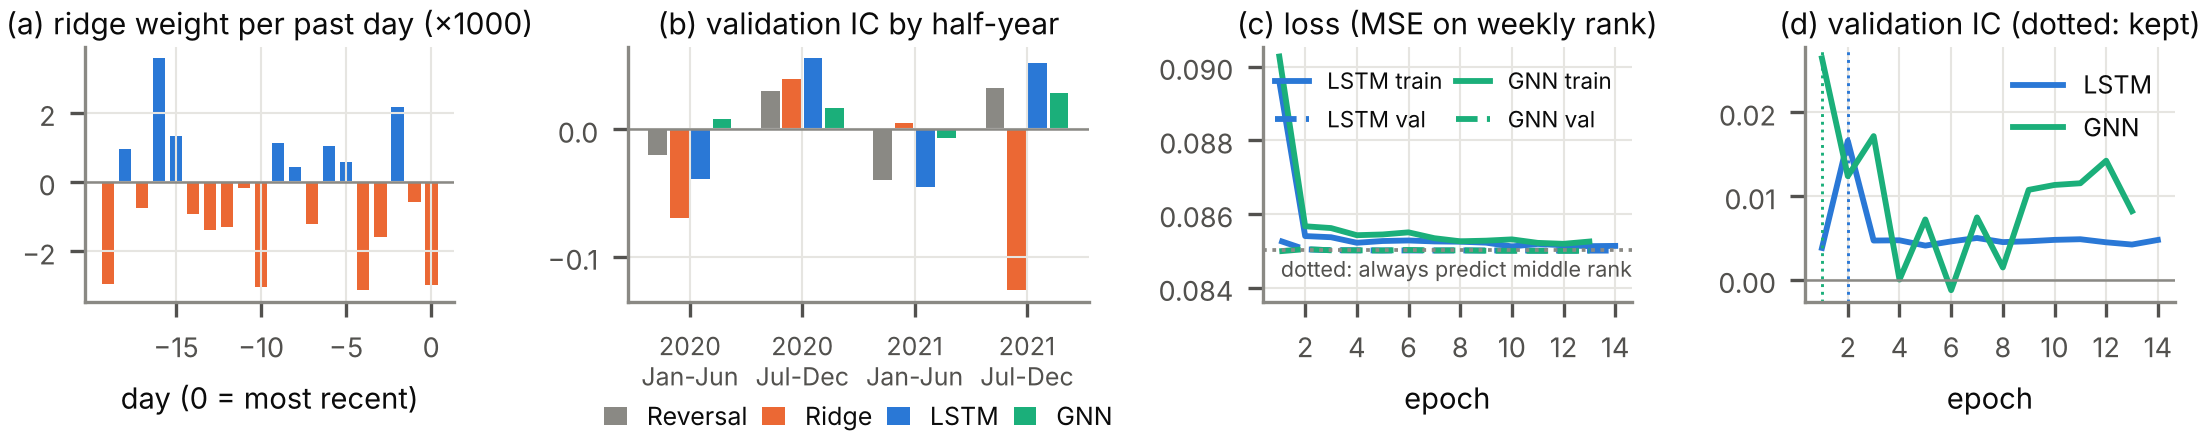
\includegraphics[width=\textwidth]{fig_results.png}
  \caption{(a) Ridge regression weight on each of the 20 past days. (b) Validation IC by half-year. (c, d) Learning curves for one seed of the LSTM baseline and the GNN.}
  \label{fig:results}
\end{figure}

\textbf{Quantitative results:} following the feedback, success means a small but consistent rank-IC gain over the LSTM-only ablation. The full GNN reaches a validation \textbf{IC of +0.0117} against +0.0058 for the LSTM baseline, and the correlation-only GNN does best at \textbf{+0.0195}, the only model above momentum (Table~\ref{tab:results}). No neural model's $t$-statistic exceeds 1 (1.1 for the weekly IC gap between the correlation-only GNN and the LSTM), the seed spread (up to 0.0100) matches the gaps between models, and the gain is not yet consistent: the full and correlation-only GNNs beat the LSTM in 48\% and 53\% of weeks, each in 2 of 4 half-years.

\textbf{What worked and what did not:} the pipeline works and all three graph versions beat the LSTM's validation IC. However, training loss settles just above 0.0850, the loss of always predicting the middle rank (Figure~\ref{fig:results}c), so the networks found little signal, and validation IC peaks within a few epochs (Figure~\ref{fig:results}d). After costs, only the single-link GNNs keep a positive Sharpe ratio.

\textbf{Qualitative results:} the GNN attends to sensible neighbours: Exxon to EOG, ConocoPhillips and Schlumberger, Apple to Nvidia, Microsoft and Texas Instruments, and Pfizer to Merck, Johnson \& Johnson and Abbott. But the weights are nearly equal (Exxon's top three each get 0.31), so it averages its neighbours. The two models' weekly ICs move together (correlation 0.69), but the GNN swings less (standard deviation 0.19 versus 0.25) and follows the market's direction (correlation 0.41). In the COVID crash week starting 9 March 2020 (average stock -12.3\%), the IC was -0.41 for the LSTM and -0.25 for the GNN. In the rebound week starting 23 March (+12.0\%), it was +0.29 and +0.47.



\textbf{Feasibility and next steps:} the pipeline is complete and a full run takes minutes, so finishing is feasible. Results are preliminary because early stopping used the validation weeks. Following the feedback, supply-chain links will run from customer to supplier, passing the customer's previous-week return and volume shock through a learned lag gate (the Cohen and Frazzini mechanism \cite{cohen2008economic}). I will also add relative returns and a ranking loss, stop early on the last training year, and evaluate once on the untouched test years and post-freeze data.

\newpage
\section*{References}
\bibliographystyle{ieeetr}
\renewcommand{\refname}{\vspace{-0.6cm}}
\bibliography{references}

\end{document}
